\documentclass[11pt]{article}
\usepackage{array}
\usepackage{amsmath}
\usepackage{listings}
\usepackage{xcolor}
\usepackage{booktabs}
\usepackage{setspace}
\usepackage[hidelinks]{hyperref}
\usepackage{graphicx}
\usepackage{subcaption}
\usepackage{float}
\usepackage[most]{tcolorbox} % 加载 tcolorbox 及其 listings 库
\usepackage{ulem} % 支持 \textdotbelow 命令
\definecolor{bgcolor}{RGB}{230,230,230}
\definecolor{bgcolor2}{RGB}{240,230,240}
\definecolor{licolor}{RGB}{100,100,100}
\linespread{1.2} 
\usepackage{algorithmic}
\usepackage[a4paper, left=2.5cm, right=2.5cm, top=3cm, bottom=2.5cm]{geometry}
\usepackage{ctex} 
\usepackage{fancyhdr}
\raggedbottom
\pagestyle{fancy}
\lhead{\textbf{Linhy\&Mayz}}
\chead{Database for Marketing Department}
\rhead{CS307 Proj1}

\newtcblisting{commandline}{
  breakable,                     % 允许代码块跨页
  colback=bgcolor,               % 背景色为灰色
  colframe=licolor,              % 边框色同背景色（若想显示
  listing only,
  arc=5mm,                       % 设置圆角半径
  boxrule=1pt,                   % 不显示边框线，如需要可调大此数值
  left=6pt, right=6pt, top=6pt, bottom=6pt, % 设置内边距
}
\newtcblisting{codeline}{
  breakable,                     
  colback=bgcolor2,               
  colframe=licolor,              
  listing only,                  
  arc=5mm,                       
  boxrule=1pt,                   
  left=5pt, right=5pt, top=5pt, bottom=5pt, 
  listing options={
    basicstyle=\ttfamily\fontsize{10pt}{11pt}\selectfont,         % 代码字体
    language=bash,                
    showstringspaces=false,       
    aboveskip=3mm, belowskip=3mm, % 上下间距
    columns=flexible,             % 让字体对齐
    keepspaces=true,
    escapeinside={(*@}{@*)},      % 允许使用 LaTeX 命令
    numbers=none,
    frame=none,
  },
  before=\setstretch{0.8},        % 设置行间距 1.5 倍
}

\title{\textbf{A Database for the Marketing Department}}
\author{} % 清空默认作者区
\date{}   % 清空默认日期区

% 自定义标题布局
\makeatletter
\renewcommand{\maketitle}{
  \begin{center}
    {\LARGE \@title \par} % 标题
    \vspace{1em}
    \textbf{\@author}     % 原作者区（可保留）
    \vspace{1em}
    \begin{tabular}{ll}
      Student ID: & 12313216, 12310908 \\
      Name:       & 林鸿渝/Linhy, 马彦昭/Mayz \\
      Course:     & CS307: Principles of Database Systems \\
      Lab:       & 2-78 Zhu  \\
      Date:       & \today
    \end{tabular}
    \vspace{0.5em}
    \hrule height 0.8pt % 分隔线
  \end{center}
}
\makeatother

\makeatletter
\renewcommand{\abstractname}{\ignorespaces}
\makeatother

\begin{document}
\thispagestyle{empty}
\maketitle


{
\setstretch{1.2}
\tableofcontents
}
\vspace{3em}

\section{任务划分及贡献}

\begin{table}[H]
  \centering
  \label{tab:customer_info}
  \renewcommand{\arraystretch}{1} % 保持之前的行间距调整
  \begin{tabular}{@{} >{\centering\arraybackslash}m{1.5cm} >{\centering\arraybackslash}m{9.5cm} >{\centering\arraybackslash}m{1.5cm} @{}}
    \toprule
    \textbf{成员} & \textbf{任务} & \textbf{贡献比} \\
    \midrule
    林鸿渝 & ER图绘制、Python实现数据导入、不同平台性能测试、trigger对于性能的影响 & 50\% \\
    马彦昭 & Java实现数据导入、Java实现多方法  & 50\% \\
    * & 报告书写、构建建表语句、方法优化、\par 导入数据量对于性能的影响 & * \\
    \bottomrule
  \end{tabular}
\end{table}

\section{实体-关系图绘制}

\begin{figure}[H]
  \centering
  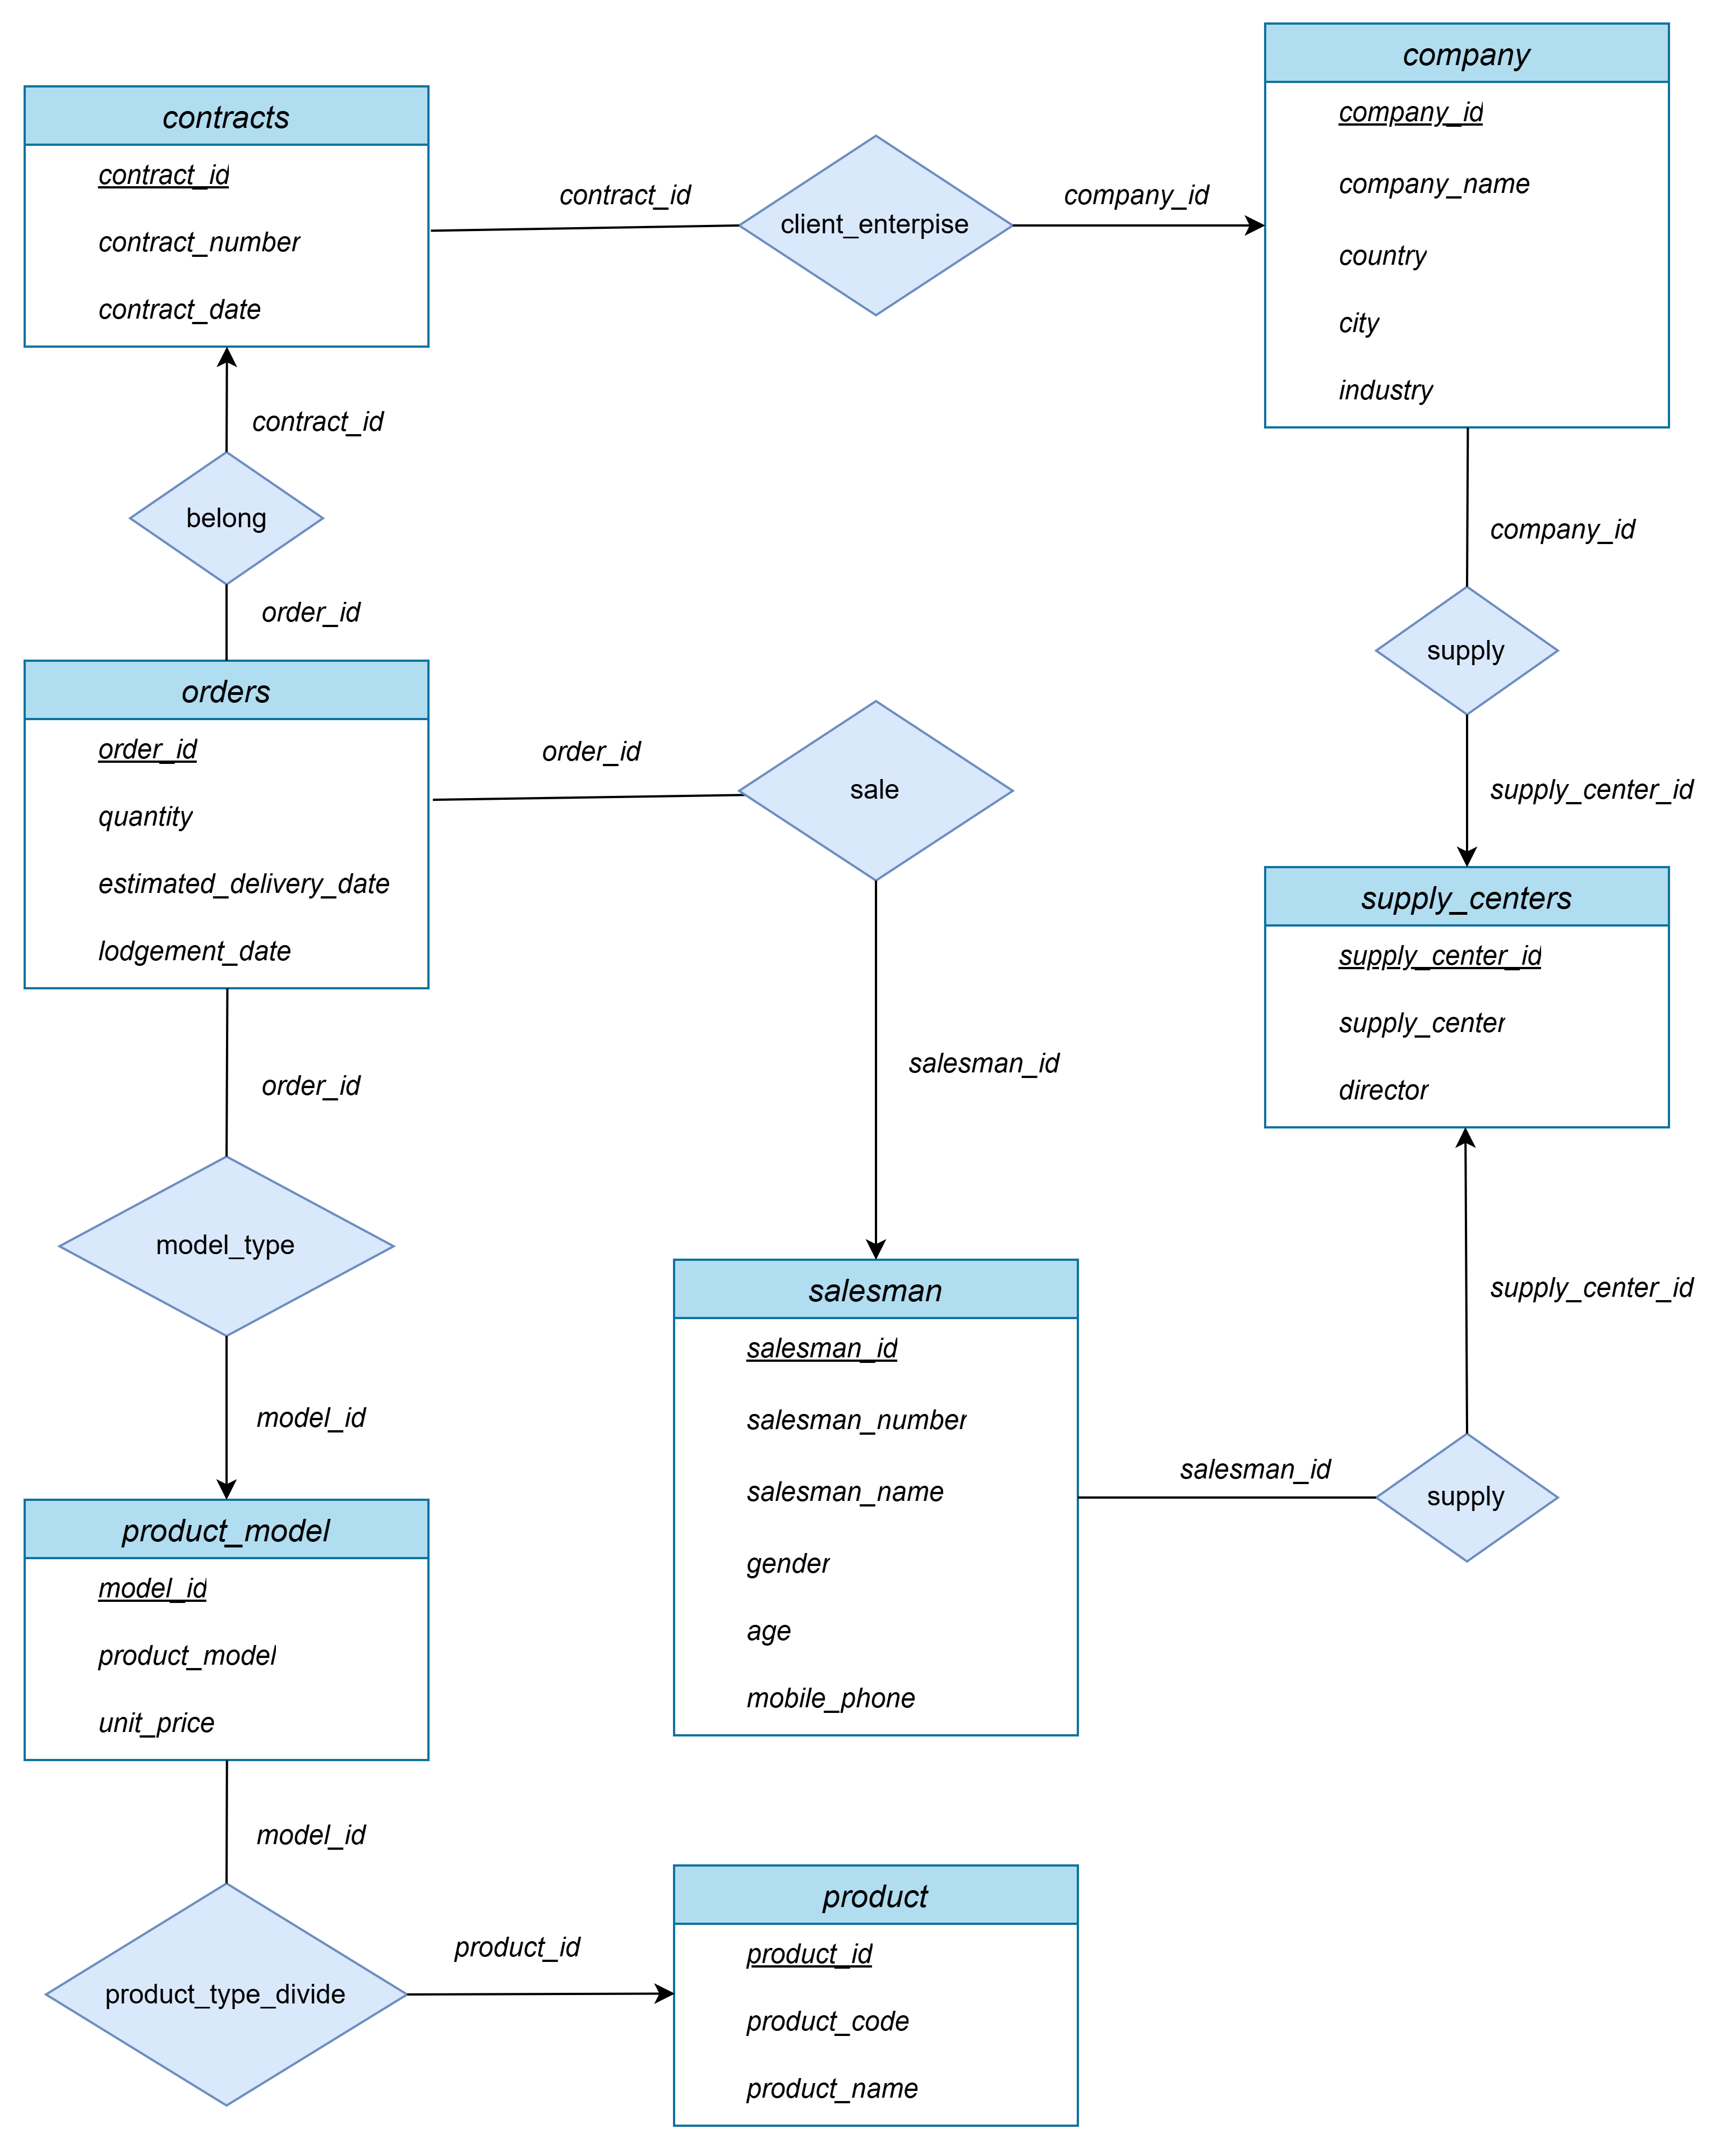
\includegraphics[width=0.7\textwidth]{ER.png}
  \caption{ER图}
  \label{fig:er_diagram}
\end{figure}

\text{本ER图通过“draw.io”工具辅助绘制（https://www.drawio.com/）}


\section{数据库设计}
\subsection{Datagrip生成图}
\begin{figure}[H]
  \centering
  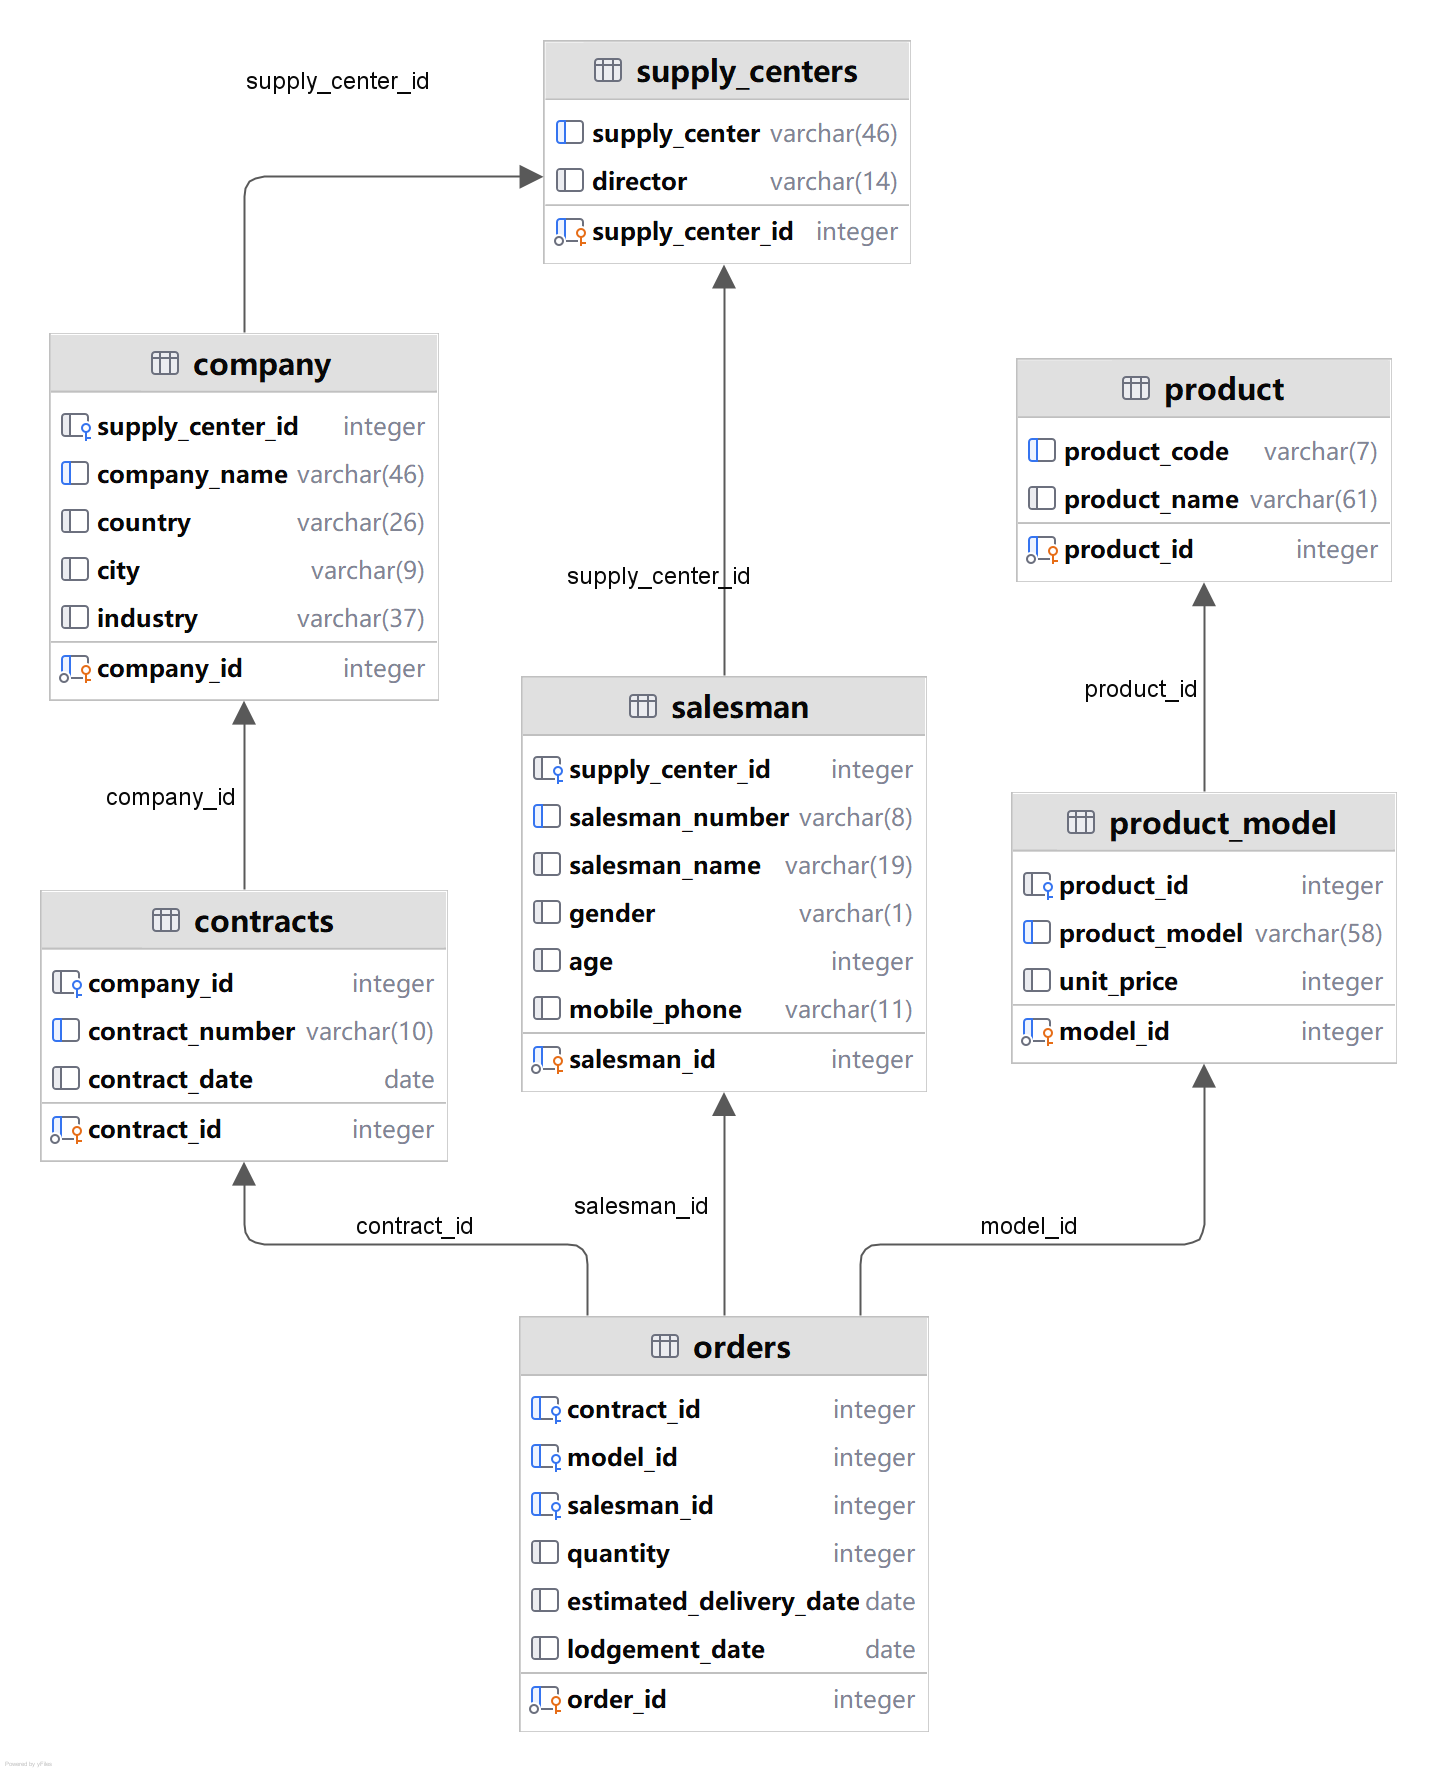
\includegraphics[width=0.7\textwidth]{ER_DATAGRIP.png}
  \caption{Datagrip生成图}
  \label{fig:datagrip_diagram}
\end{figure}

\subsection{数据库设计简述}
\subsubsection{数据描述}
本数据库以Output25S.csv为基础建立。在原始的csv文件中，包含了500,000条数据，即500,000条订单。任意订单均包含合同编号(contract\_number)、客户公司(client\_enterprise)、公司所在国家(country)、城市(city)、所属行业(industry)、产品编号(product\_code)、产品名称(product\_name)、产品型号(product\_model)、产品型号对应单价(unit\_price)、订单产品数量(quantity)、合同下单日期(contract\_date)、产品预计到达日期(estimated\_delivery\_date)、实际到达日期(lodgement\_date)、公司所在区域管理员(director)、公司所在区域的供应中心(supply\_center)、销售员(salesman)、销售员编号(salesman\_number)、性别(gender)、年龄(age)、电话(mobile\_phone)，共计20类属性。\par
\hspace{0em}其中，若客户公司不在中国，其所在城市(city)对应值可为NULL；若实际送达日期(lodgement\_date)在2025-3-24之后，则该值也可为NULL。\par
\hspace{0em}导入数据的类型已在生成图中展示，报告空间有限，不再赘述。
\subsubsection{属性划分}
\textbf{1NF：}所有字段均为\textbf{原子值}。Output25S.csv中所有属性均为原子属性，且没有重复的列，因此满足1NF。\par
\textbf{2NF：}非主键字段\textbf{完全依赖}于主键。由此将原表格划分为以下子表：\par

\begin{table}[H]
  \centering
  \label{tab:customer_info}
  \renewcommand{\arraystretch}{1} % 保持之前的行间距调整
  \begin{tabular}{@{} >{\centering\arraybackslash}m{2.5cm} >{\centering\arraybackslash}m{12cm} @{}}
    \toprule
    \textbf{子表} & \textbf{属性} \\
    \midrule
    订单 & \underline{订单ID}、订单产品数量、预计到达日期、实际到达时期  \\
    合同 & \underline{合同ID}、\dotuline{合同编号}、合同签署时间\\
    公司 & \underline{公司ID}、\dotuline{公司名}、公司所在国家、城市、所属行业\\
    销售员 & \underline{销售员ID}、\dotuline{销售员编号}、姓名、性别、年龄、电话\\
    产品型号 & \underline{产品型号ID}、\dotuline{产品型号}、型号单价\\
    产品 & \underline{产品ID}、\dotuline{产品编号}、产品名称\\
    供应中心 & \underline{供应中心ID}、\dotuline{供应中心名称}、{所在区域管理员}\\
    \bottomrule
  \end{tabular}
\end{table}

\textbf{3NF:}非主键字段中不能有\textbf{传递依赖}。检查上表，所有子表的元素都直接与主键(ID)相关，所有非主键字段都直接依赖于主键，不是通过其他非主键字段间接依赖。\par\nopagebreak[4]

\subsubsection{约束条件}
\textbf{主键约束：}所有子表主键均为子表对应ID，已在上表中以下划线标注。\par
\textbf{外键约束：}3.2.2属性划分下的表中不包含外键属性。在此部分加入。定义一对多关系：R(1,x), 我们可找到如下表间关系：(supply\_centers, company), (supply\_centers, salesman), (company, contracts), (product, product\_model), (contracts, orders), (salesman, orders), (product\_model, orders)。以此一对多关系连接不同子表，足够实现完整数据库，无需创建中间表声明表间关系。\par

\begin{table}[H]
  \centering
  \label{tab:customer_info}
  \renewcommand{\arraystretch}{1} % 保持之前的行间距调整
  \begin{tabular}{@{} >{\centering\arraybackslash}m{2.5cm} >{\centering\arraybackslash}m{12cm} @{}}
    \toprule
    \textbf{子表} & \textbf{外键(指向表)} \\
    \midrule
    订单 &  \dotuline{合同ID}(contracts)、\dotuline{销售员ID}(salesman)、\par \dotuline{产品型号ID}(product\_model) \\
    合同 & 公司ID(company)\\
    公司 & 供应中心ID(supply\_center)\\
    销售员 & 供应中心ID(supply\_center)\\
    产品型号 & 产品ID(product)\\
    \bottomrule
  \end{tabular}
\end{table}

\textbf{唯一约束：}所有表格均有唯一约束。除去orders表，其余子表Unique约束均已在表2中以加点形式标明。orders表以三个外键作为联合Unique约束，已在上表以加点形式标注。\par



\section{数据导入}
\subsection{数据导入说明}
\subsubsection{数据修改说明}
原csv文件中，存在错误数据使得同一销售员编号对应不同销售员。
\begin{figure}[H]
  \centering
  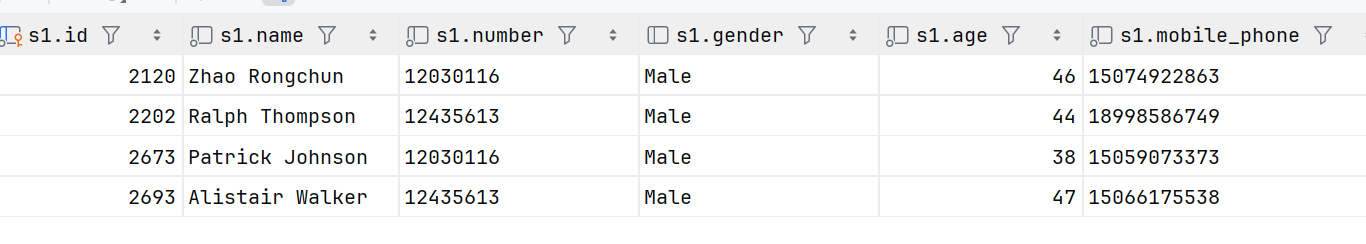
\includegraphics[width=1\textwidth]{Modify.png}
  \caption{通过Cross join找到的错误数据}
  \label{fig:wrong_data}
\end{figure}
进行数据库构建时，我们对所有含有上述字段的数据进行如下修改:
\begin{codeline}
...  Patrick Johnson 12030116 ... → ... Patrick Johnson 12313216 ...
...   Ralph Thompson 12435613 ... → ... Ralph Thompson  12310908 ...
\end{codeline}

\subsubsection{脚本使用说明}
\begin{table}[H]
  \centering
  \label{tab:customer_info}
  \renewcommand{\arraystretch}{1} % 保持之前的行间距调整
  \begin{tabular}{@{} >{\centering\arraybackslash}m{3.5cm} >{\centering\arraybackslash}m{2cm}>{\centering\arraybackslash}m{10cm} @{}}
    \toprule
    \textbf{Script Name} & \textbf{Author} & \textbf{Description} \\
    \midrule
    App.java & Mayz & 运行该程序，先初始化数据库与Reader，再创建与表一一对应的语句，对每个语句单独计算缓冲大小，逐行完成数据载入\\
    \midrule
    DBConnection.java & Mayz & 读取配置文件并初始化数据库连接\\
    \midrule
    StatementPreparer.java & Mayz & 对语句使用提供基本支持，如使用JDBC的缓冲方法、对不同的目标数据类型自动选择处理方式\\
    \midrule
    InsertMethods.java & Mayz & 静态类，完成对从文件中读取数据的处理，如去重，添加ID等，将其整合后注入insert语句中\\
    \midrule
    MyUsedSQLs.java & Mayz & 枚举类，存储sql语句，方便改，查\\
    \midrule
    UsedDataType.java & Mayz & 枚举类，用于作为参数传递需要填入表中的数据类型\\
    \bottomrule

  \end{tabular}
\end{table}

\hspace{-2em} \textbf{具体导入流程：}\par
\hspace{-1em}1. 读取配置文件，连接数据库，读取原始数据文件\par
\hspace{-1em}2. 执行清理建表语句，创建不同表的PrepareStatement对象，并用数组存储PrepareStatement对象。\par
\hspace{-1em}3. 使用while循环，逐行读取csv文件，按照外键依赖，顺序执行batch条件判断\par
\hspace{-1em}4. 结束循环，最后执行一次提交语句，确保不漏，关闭reader和连接，计时\par

\subsection{导入数据准确性验证}
\subsubsection{postgreSQL查询语句}
\begin{commandline}
-- 1. 不同性别的销售员分别有多少个
select distinct gender, count(distinct salesman_name)
from salesman
group by gender;

-- 2. 每一个supply center中有多少公司
select supply_center, count(distinct company_name)
from company
         join supply_centers on company.supply_center_id = supply_centers.supply_center_id
group by supply_center
order by supply_center ASC;

-- 3. 每一个supply center中有多少销售员
select s.supply_center, count(distinct salesman_id)
from supply_centers s
         join salesman m on s.supply_center_id = m.supply_center_id
group by s.supply_center
order by supply_center ASC;

-- 4. 年龄在某个上界或下界区间的销售员有多少个
select count(distinct salesman)
from salesman
where age > 42 and age < 45;

-- 5. 每一个supply center中有多少国家
select s.supply_center, count(distinct country)
from company c
         join supply_centers s on c.supply_center_id = s.supply_center_id
group by s.supply_center
order by supply_center ASC;

-- 6. 根据某一个国家名称，列出其所有的公司名称，及其公司所属行业
select distinct country, company_name, industry
from company
where country = 'Italy'
order by country, company_name;

-- 7. 根据某一个产品编码，列出其所有的产品型号、及对应的单价
select distinct p.product_code, m.product_model, m.unit_price
from product p
         join product_model m on p.product_id = m.product_id
where product_code = 'B56K283'
order by p.product_code, m.product_model, m.unit_price;

-- 8. 根据某一个合同编码，列出合同中所有订单内容，
每个订单包含（产品型号、购买数量、销售员名称、实际到达日期）
select distinct c.contract_number, p.product_code, m.product_model, o.quantity, s.salesman_name, o.lodgement_date
from contracts c
         join orders o on c.contract_id = o.contract_id
         join salesman s on o.salesman_id = s.salesman_id
         join product_model m on o.model_id = m.model_id
         join product p on m.product_id = p.product_id
where contract_number = 'CSE0000267'
order by c.contract_number, m.product_model, o.lodgement_date, s.salesman_name, o.lodgement_date;

\end{commandline}

\subsection{导入方式拓展}

\textbf{本拓展的环境及配置均详见 4.3.4 中的 Window系统栏目}

\subsubsection{多语言导入：Python}
\begin{table}[H]
  \centering
  \label{tab:customer_info}
  \renewcommand{\arraystretch}{1} % 保持之前的行间距调整
  \begin{tabular}{@{} >{\centering\arraybackslash}m{4cm} >{\centering\arraybackslash}m{1.5cm}>{\centering\arraybackslash}m{10cm} @{}}
    \toprule
    \textbf{Script Name} & \textbf{Author} & \textbf{Description} \\
    \midrule
    LoadInStages.py & Linhy & 运行该py文件完成数据导入\\
    \midrule
    DbConnection.py & Linhy & 读取配置文件进行数据库连接与关闭，获取cursor及con\\
    \midrule
    InsertMethod.py & Linhy & 结合不同sql的PrepareStatement对象，提供不同Insert语句对应的插入方法。与此同时维护一个字典(Hash)，便于之后添加不同表内的主键id\\
    \midrule
    PrepareStatement.py & Linhy & 每个语句对应一个pstmt，维护sql语句以及参数数组\\
    \midrule
    DataType.py & Linhy & 枚举类，作为pstmt传入参数的类型选择，进行不同if语句\\
    \midrule
    SqlSentences.py & Linhy & 不同sql语句，包括建表删表以及插入数据、增加约束\\
    \bottomrule
  \end{tabular}
\end{table}

\hspace{-2em} \textbf{具体导入流程：}\par
\hspace{-1em}1. pandas读csv文件，并进行预处理，删除最后一行以及将‘’和nan转为None。\par
\hspace{-1em}2. 读取配置文件，连接数据库，获取stmt(cursor)及con。\par
\hspace{-1em}3. 给所有sql语句，包括建表删表以及插入数据、增加约束，创建PrepareStatement对象。\par
\hspace{-1em}4. 删除所有已有的表，创建数据库设计的7个表格，create语句中已添加约束。为下面插入数据做初始准备。\par
\hspace{-1em}5. 逐行读取csv文件，先向supply\_center以及product这两个完全没有外键约束的表格插入数据。具体实现为：调用InsertMethod的插入方法，存至对应pstmt的参数数组，当执行数量达到batch便执行executemany。commit提交后clear参数数组。最后统一再commit一次，处理余数。\par
\hspace{-1em}6. 同样的实现逻辑，依次插入有上述两张表的外键依赖的：salesman、product\_model、company。再插入依赖company的contracts。最后插入orders。\par

\hspace{-1em}\par
Python实现的方式与Java有所不同，Java是把一行数据拆分到每条指令，处理后先execute放入缓存区，在统一commit。而Python是把每个数据分了四个阶段分别放入缓存区，且sql语句之间不再允许交叉。原始的Java代码在每次插入数据均调用executeUpdate，非常低效，本Python实现使用executemany实现批量导入，减少与数据库间的访问次数，与Java第二次优化使用的addBatch类似。下面与Java第二次优化的导入性能做对比：\par
\hspace{-1em}\par
\hspace{2em}\textbf{Java第二次优化：25181 records/s\ \ \ \ Python原始：11055 records/s}\par
\hspace{-1em}\par
我们发现，Java的addBatch竟然比Python的executemany快了近一倍？！查阅资料发现Python调用的psycopg2的executemany是伪批量操作，实际是循环插入，性能与execute接近。对比Java原始的效率，为13378 records/s，与Python接近，再加上Python的运行时开销比Java大，这样的结果符合预期。

\subsubsection{导入优化}
\begin{itemize}
  \item \textbf{Java:} \par
\hspace{-2em}\textbf{初始版本：}参照基础的方法，在InsertMethods.java中使用hashmap将主键和生成的ID对应并完成去重，每次缓冲区满统一执行。\par
\hspace{-2em}\textbf{第一次优化：}在InsertMethods.java将主键优先提取，避免重复提取主键的操作；在App.java中调用InsertMethods中下一次要赋的ID作为数据量，将各语句分别计算缓冲。\par
\hspace{-2em}\textbf{第二次优化：}经过进一步学习JDBC，在StatementPreparer.java中将原先的update方法改为addBatch方法，并在App.java中加入executingXXX方法，方便嵌套调用，避免出现执行batch时相关语句未提交的错误。\par
\hspace{-2em}\textbf{第三次优化：}进一步优化了分别缓冲的逻辑，在StatementPreparer.java中加入了一个int数据标记batch中的数据量，加入了batch为空的逻辑判断语句，减少了重复执行空batch的次数。\par
\end{itemize}

从“(a)Java优化”可得，第一次优化改变了将原始数据的记录改变为目标表中记录的逻辑，变为统一处理主键，通过各语句分别缓冲，减少了提交代码的次数，得到了大约14\%的效率优化；第二次优化替换JDBC执行方法，利用PreparedStatement的批量操作特性并引入嵌套提交逻辑，消除没有对应外键的约束错误，得到了大约65\%的效率优化；第三次优化改变提交语句的判断条件，更严格的限制了执行，减少了不必要的执行，避免了执行空batch，得到了大约92\%的效率优化；总体而言，Java优化主要聚焦于数据库交互层面的深度重构。前两次优化通过重构主键处理流程和JDBC批处理机制，实现了事务级的性能提升。第三次优化通过引入批量标记与空操作检测机制，精准控制数据库写入流程，消除空批处理的性能开销。最终实现了约3倍的性能提升。

\begin{figure}[H]
  \centering
  \begin{subfigure}{0.48\textwidth}
    \centering
    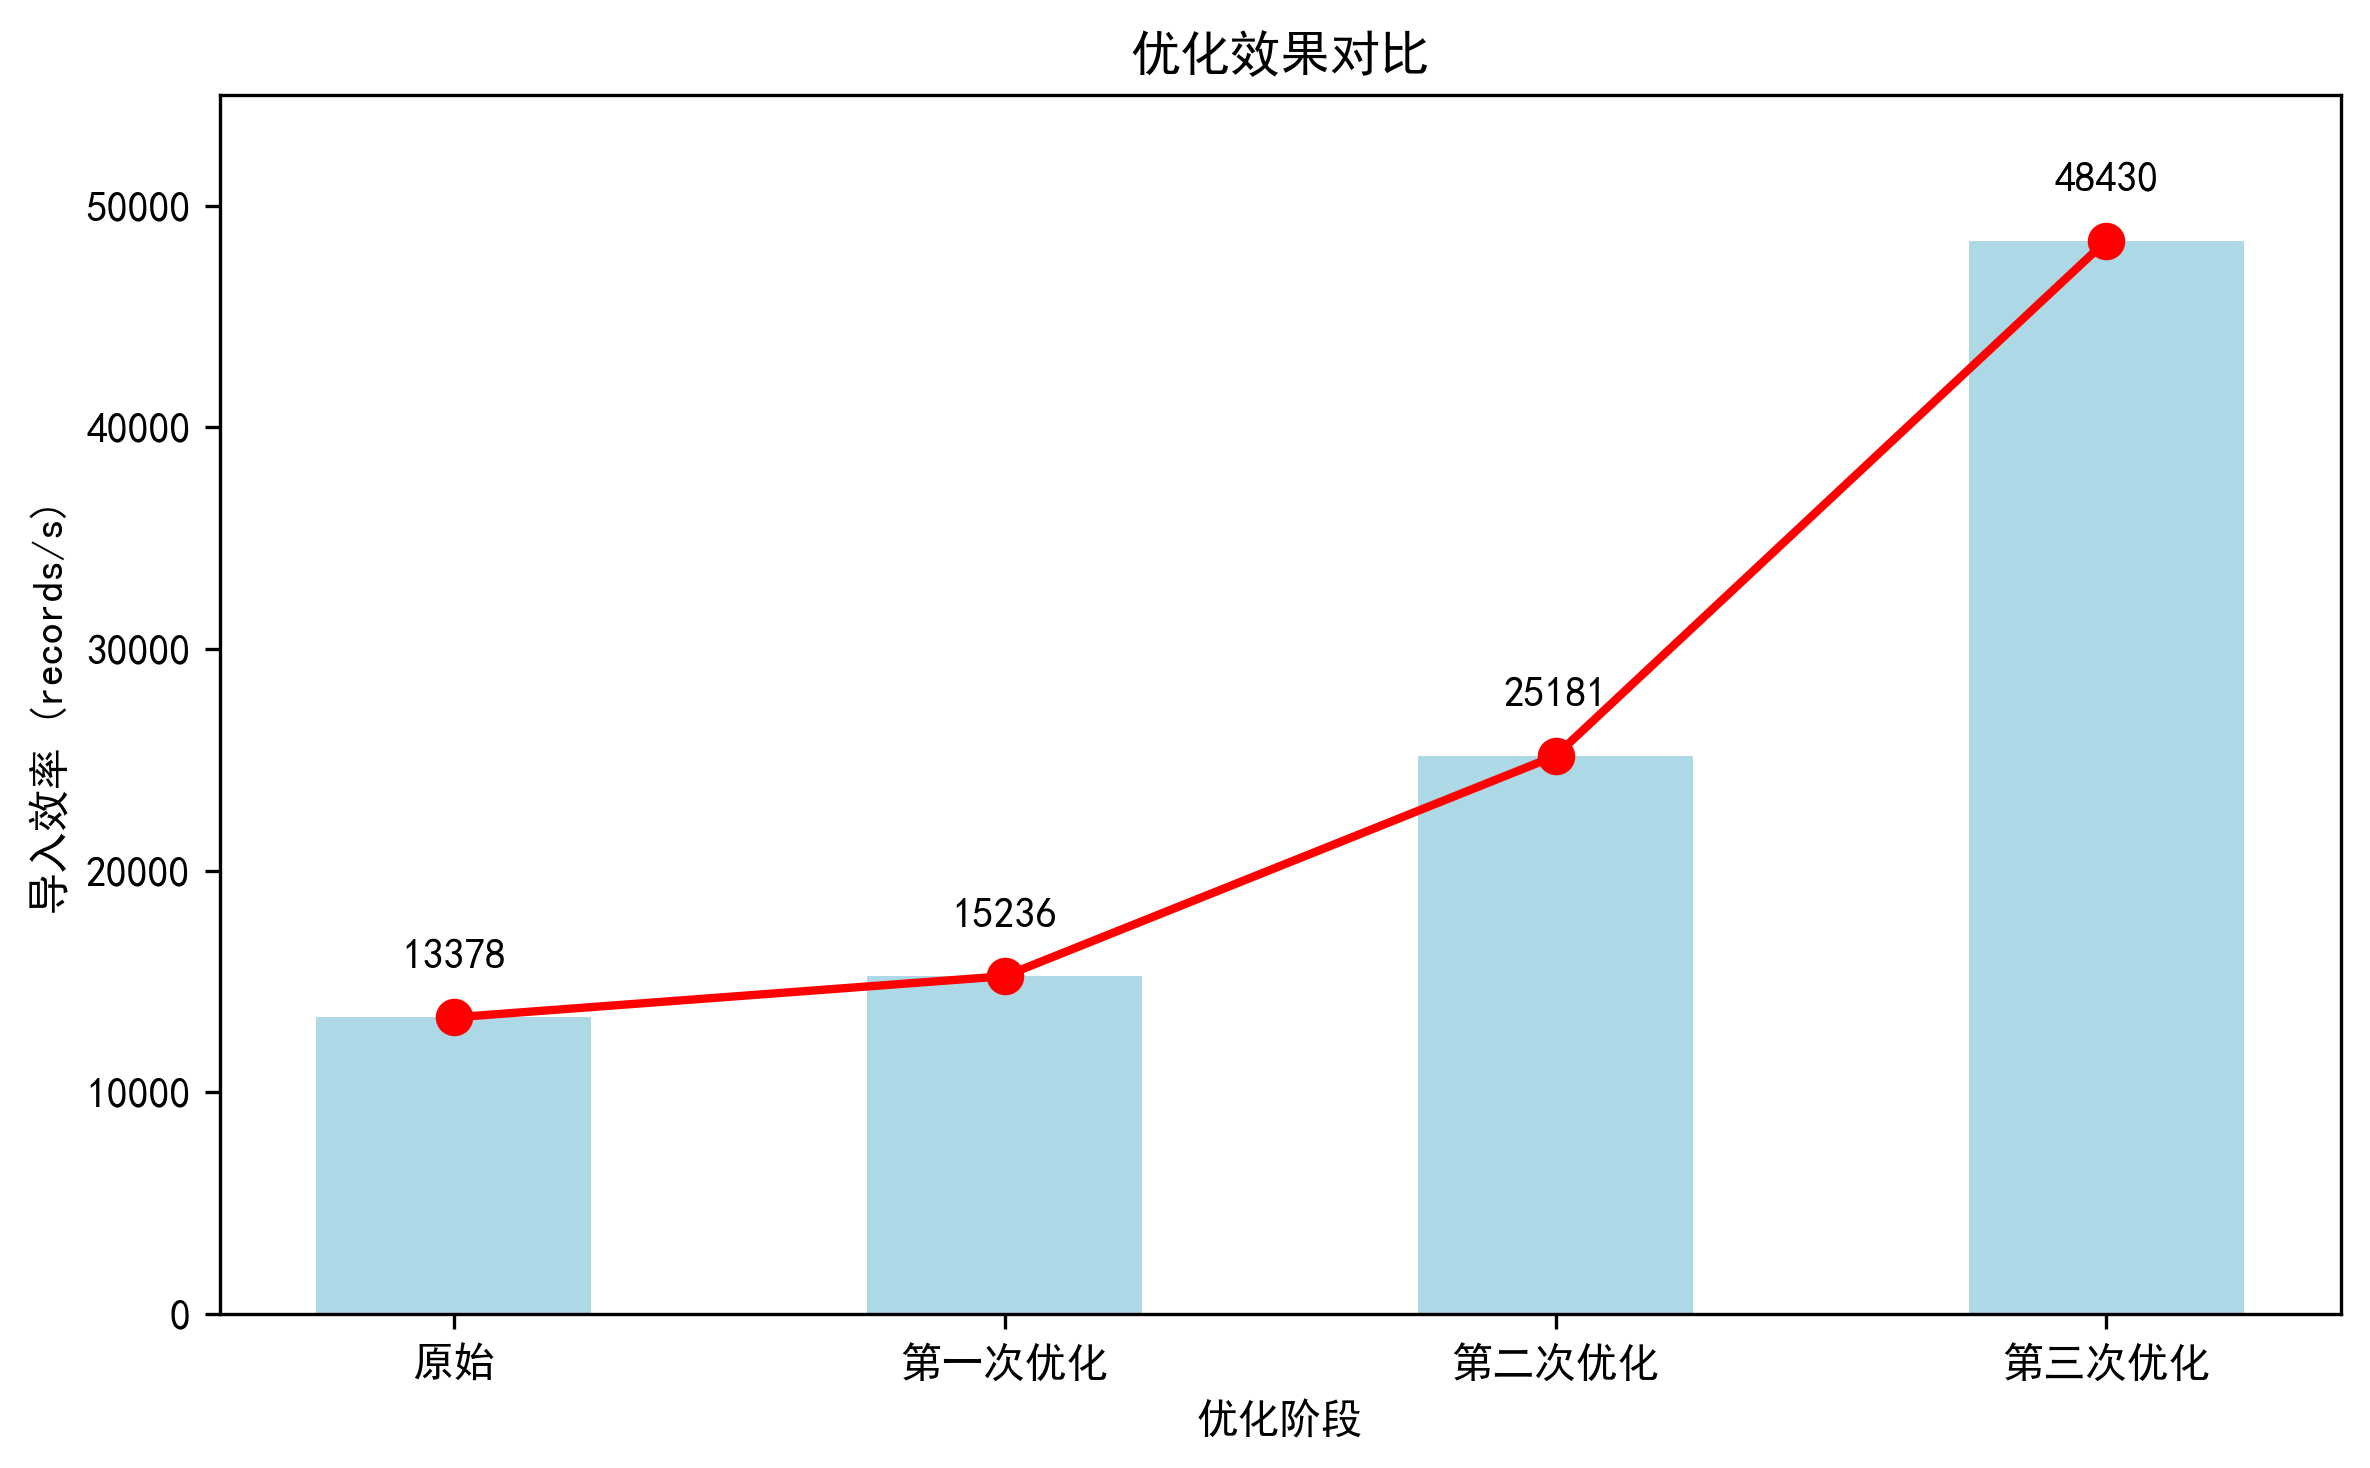
\includegraphics[width=\textwidth]{java_opt.png}
    \caption{Java优化}
    \label{fig:java_opt}
  \end{subfigure}
  \hfill
  \begin{subfigure}{0.48\textwidth}
    \centering
    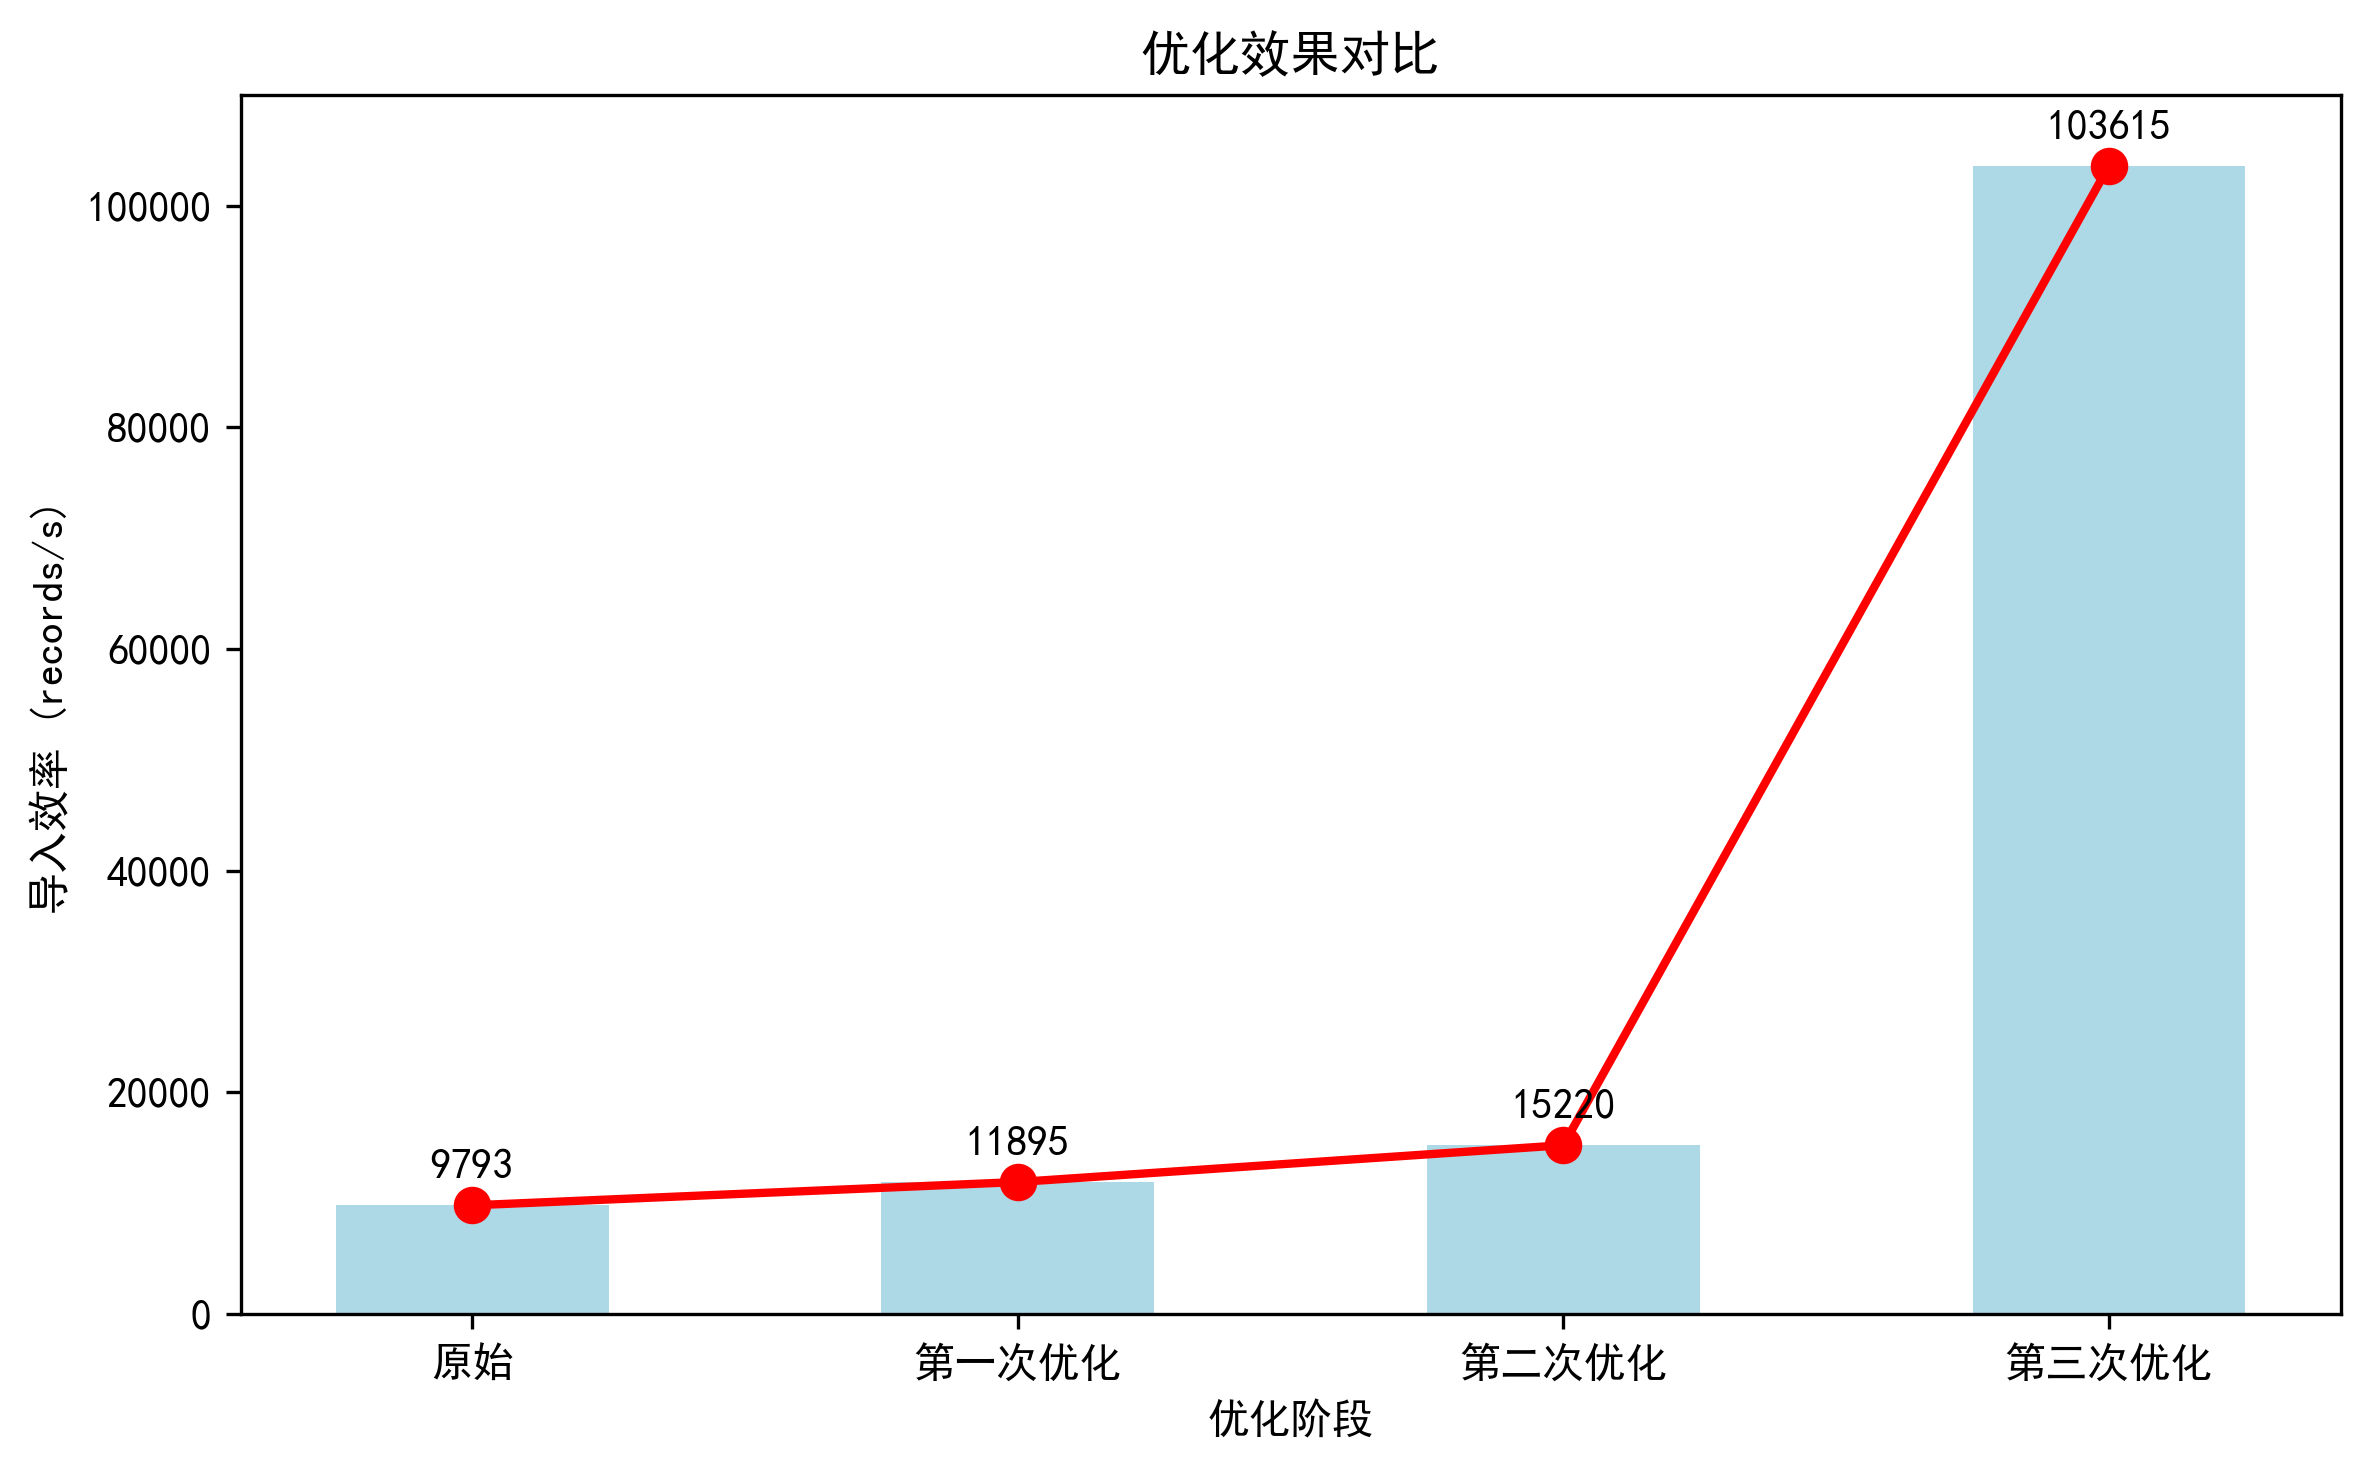
\includegraphics[width=\textwidth]{py_opt.png}
    \caption{Python优化}
    \label{fig:py_opt}
  \end{subfigure}
  \caption{Java与Python优化对比}
  \label{fig:opt_comparison}
\end{figure}

\begin{itemize}
\item \textbf{Python:} \par
\hspace{-2em}\textbf{初始版本：}先导入supply\_center, product两张无外键的独立表，再导入salesman, product\_model, company三张存在关于上一张表的外键约束的表格，随后导入依赖company的contracts，最后导入orders。\par
\hspace{-2em}\textbf{第一次优化：}初始版本建表时便添加外键及唯一约束，分四个阶段导入，每次都需重新读取数据，以及检查约束条件。本方法采取先建表，不进行任何约束，最后统一添加外键与唯一约束。\par
\hspace{-2em}\textbf{第二次优化：}直至第一次优化，都需要用到PrepareStatement.py文件，每次都要对不同的sql语句创建pstmt对象，并进行访问，较为耗时。将其删去，对InsertMethod进行修改，将其内部方法的pstmt变量改为list，将要修改的变量存入list，而不是pstmt.list。\par
\hspace{-2em}\textbf{第三次优化：}上述三个导入方式均采用 psycpg2.cursor.executemany() 来导入，现换为copy方法，通过copy\_expert和StringIO将pandas数据帧写入数据库。\par
\end{itemize}

从“(b)Python优化”可得：第一次优化延迟了约束检查，减少了约束验证开销，有21.4\%的提升，效果明显；第二次优化移除了PSTMT，使用list直接存储SQL要修改的变量，减少Python层面的计算和内存开销，提升了32.4\%的性能；第三次优化使用copy命令，从根本上消除了逐条插入的开销，如SQL解析、网络往返，插入效率提升580.9\%。总体而言，前两次优化基于Python层面，提升有限，而第三次优化的copy命令在数据库层面，直接将数据流式写入PostgresSQL的存储层，绕过SQL解析和逐条事务写入，数据加载后再统一处理索引和约束，开销极低。除此之外，使用顺序I/O而不是随机I/O，即数据按顺序写入文件的末尾，形成连续的数据块。这种写入模式，磁盘只需要在文件末尾连续追加数据，无需频繁跳转到不同的磁盘位置。


\subsubsection{Java实现的另一导入方式}
\begin{table}[H]
  \centering
  \label{tab:customer_info}
  \renewcommand{\arraystretch}{1} % 保持之前的行间距调整
  \begin{tabular}{@{} >{\centering\arraybackslash}m{4cm} >{\centering\arraybackslash}m{1.5cm}>{\centering\arraybackslash}m{10cm} @{}}
    \toprule
    \textbf{Script Name} & \textbf{Author} & \textbf{Description} \\
    \midrule
    GenCSVToLoad.java & Mayz & 运行该文件，载入原始数据后输出加入ID的中间表，中间表被直接不去重输入，得到重复表，使用SQL语句从重复表创建最终表\\
    \midrule
    GenID.java & Mayz & 根据主键，使用hashmap去重，生成ID\\
    \midrule
    DBConnection.java，StatementPreparer.java，MyUsedSQLs.java & Mayz & 复用部分\\
    \bottomrule
  \end{tabular}
\end{table}


\hspace{-2em} \textbf{具体导入流程：}\par
\hspace{-1em}1. 读取配置文件，连接数据库，完成初始化。\par
\hspace{-1em}2. 逐行遍历，对每一个记录单独提取主键生成ID，并生成加入ID的新记录，使用BufferedWriter缓冲后写入，生成中间表\par
\hspace{-1em}3. 逐行读取中间表，将中间表一条记录拆分成不同表的不同记录，使用单一n计数，到达batch后统一写入，生成七张未经去重的重复表\par
\hspace{-1em}4. 创建最终表，使用SELECT，DISTINCT去重后写入，得到最终表，移除重复表，关闭连接，计时\par

\hspace{-1em}\par
\hspace{2em}\textbf{Java：27967 records/s}\par

\hspace{-1em}\par
从过程中可得，这一方法总共需要遍历三次，第一次遍历读取原文件，生成中间表；第二次遍历读取中间表，将中间表中的数据重复地填入数据库中，生成重复表；第三次遍历在数据内部进行，筛选出不重复的数据，得到最终表。由于需要经历三次遍历，这一方法可以预想地，相较于边运行边去重，只遍历一次的第一种方法效率较低，且由于第二次遍历时不对数据进行筛选，重复填入，需要执行的语句数量也较优化后的第一种多上数倍，这些因素综合造成了该方法效率较低。在时间消耗上，对于50万条数据的原始数据，第一次遍历需要大致1.6秒，第二次遍历需要大致16秒，第三次遍历需要大致1.5秒。可见主要的时间消耗来源于大量访问数据库，而虽然数据量上基本等同，但得益于CSVReader，CSVWriter和postgreSQL的优化，第一，二次遍历速度较快。但该方法也有部分可取之处，使得其效率能够达到27000条每秒的水平，这主要得益于该方法逻辑较为简单，需要执行的判断较少，中间变量较少，将大量判断交由postgreSQL完成，借助postgreSQL的优化提高了自身的效率。但也正是这一思路，使得其无法优化第二次遍历的效率，导致性能受限。

\subsubsection{多平台导入}
本小节测试在Windows和MacOS上运行的性能差异。其中配置环境如下：

\begin{table}[H]
  \centering
  \label{tab:customer_info}
  \renewcommand{\arraystretch}{1} % 保持之前的行间距调整
  \begin{tabular}{@{} >{\centering\arraybackslash}m{4cm} >{\centering\arraybackslash}m{6cm}>{\centering\arraybackslash}m{6cm} @{}}
    \toprule
    \textbf{系统} & \textbf{配置} & \textbf{运行环境} \\
    \midrule
    Windows & intel i9-13900HX、16GB RAM & PostgreSQL 17.4、Python 3.11、Pandas 2.0.3、Psycopg2 2.9.9 \\
    \midrule
    MacOS & Mac M2 Max、32GB RAM & PostgreSQL 16.2、Python 3.11、Pandas 2.1.4、Psycopg2 2.9.10 \\
    \bottomrule
  \end{tabular}
\end{table}

\vspace{0em}我们在不同平台上运行了相同的导入脚本，并记录了每个平台的运行时间。以下是测试结果：

\begin{figure}[H]
  \centering
  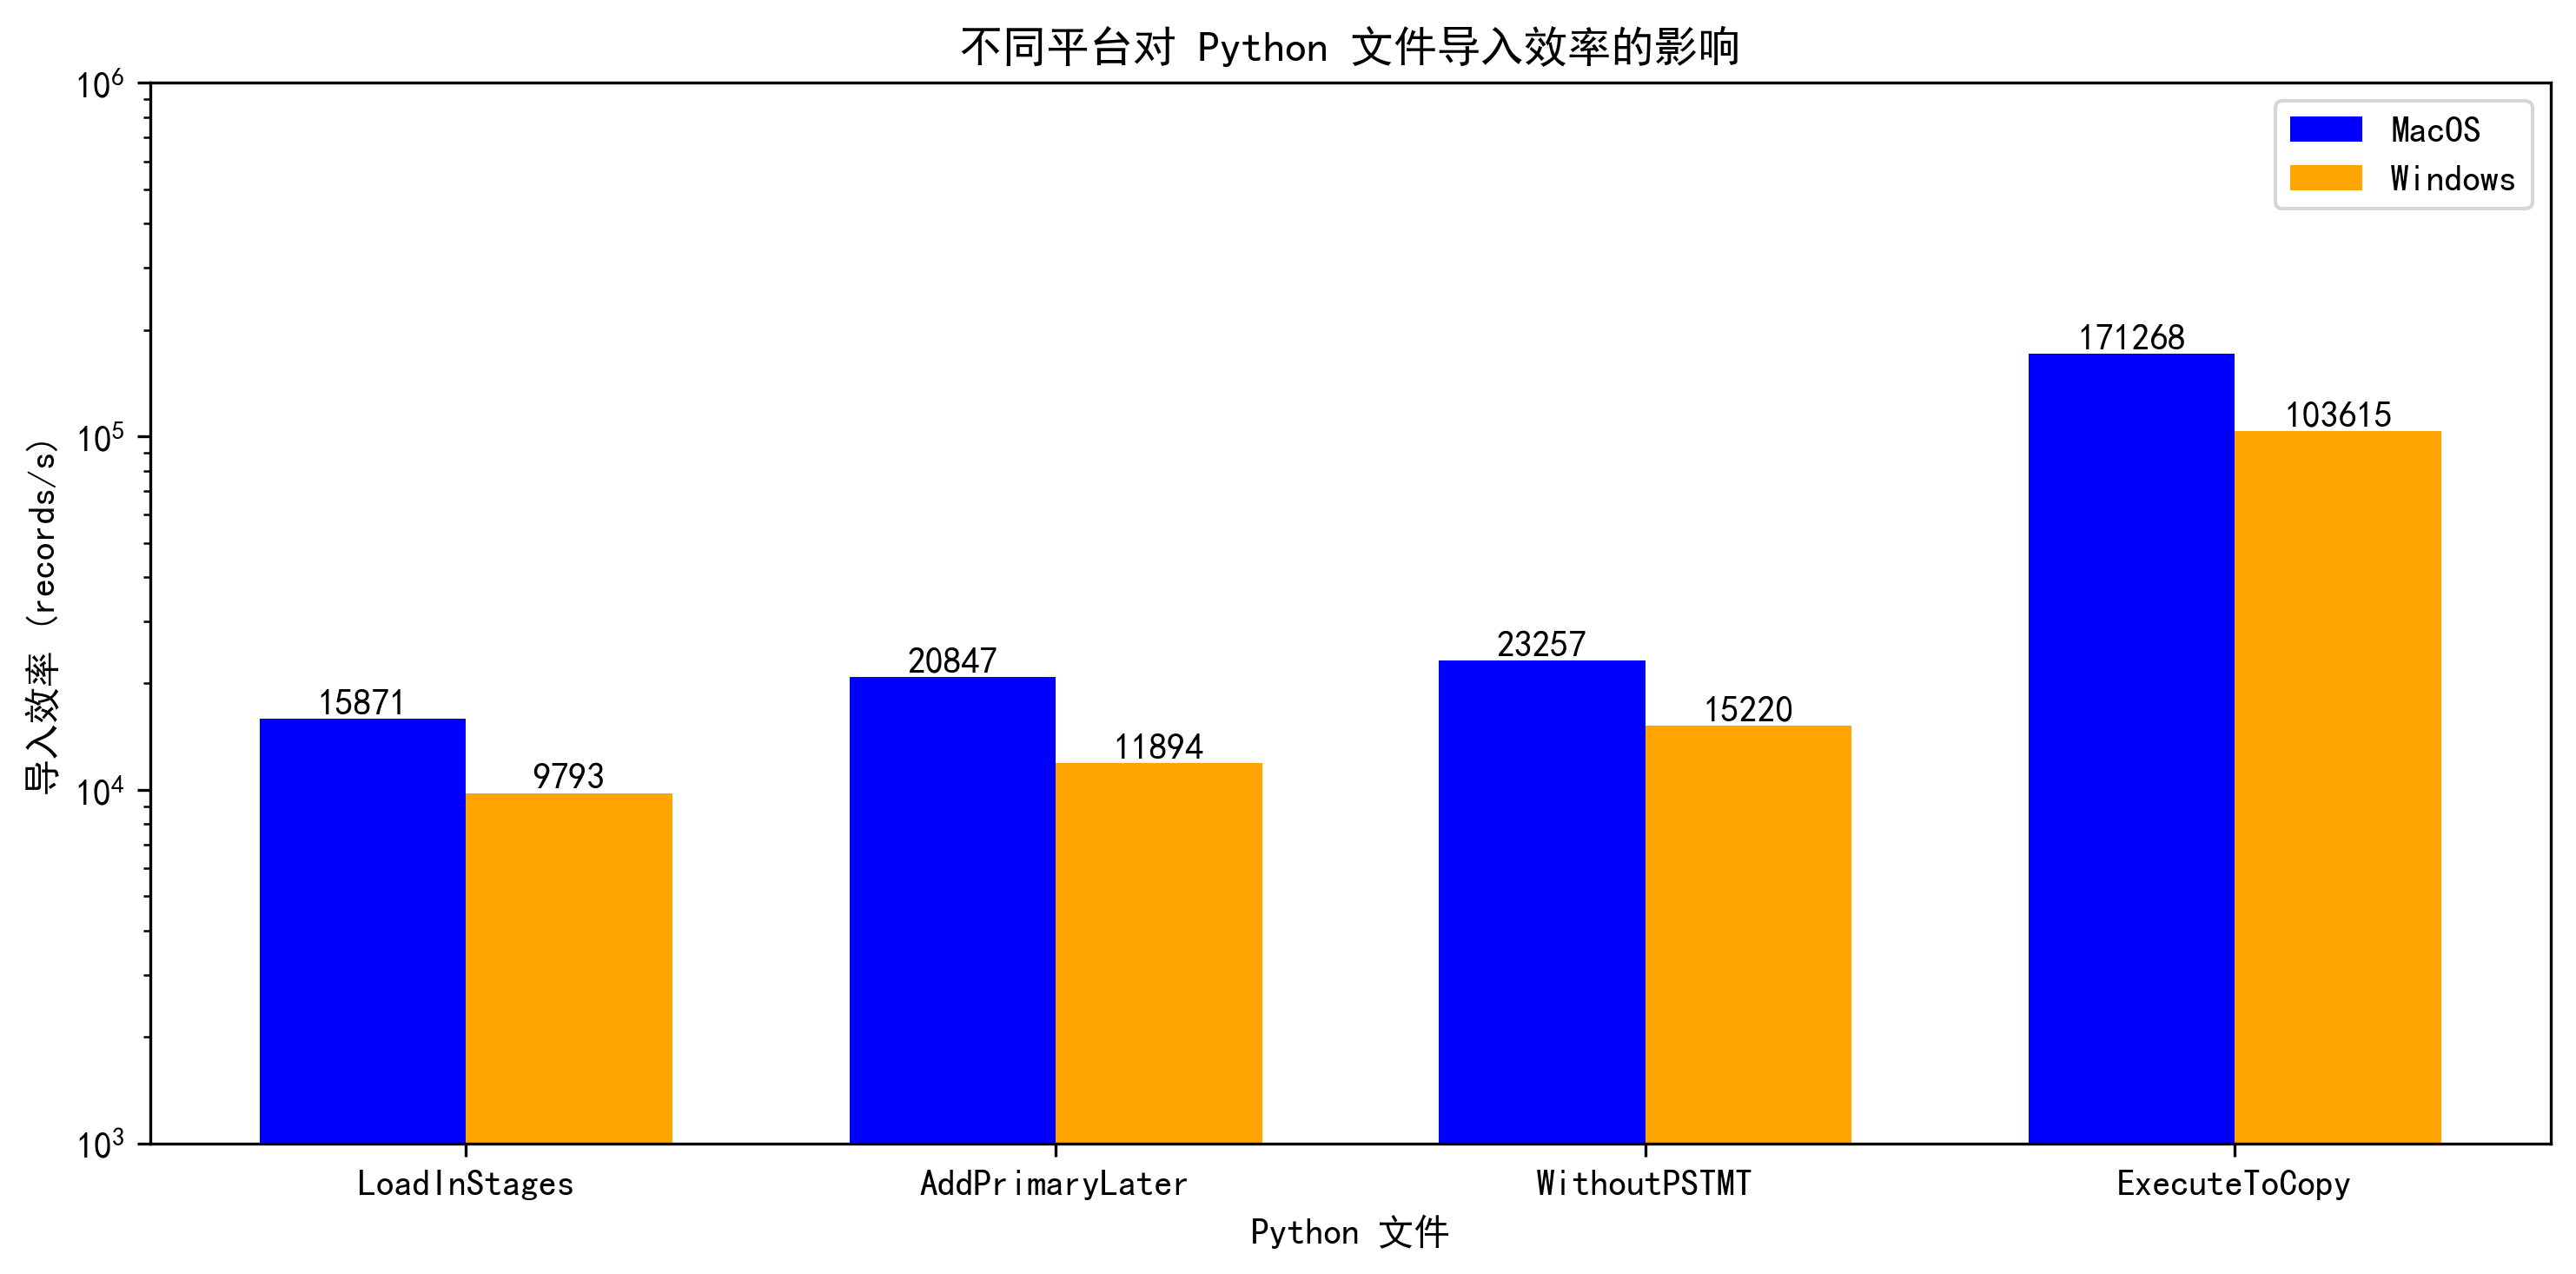
\includegraphics[width=1\textwidth]{platform.png}
  \caption{不同导入平台对于性能的影响}
  \label{fig:platform_performance}
\end{figure}

比对结果可得，MacOS的性能明显优于Windows，主要原因在于MacOS的硬件优势，其内存带宽(400GB/s)显著大于i9-13900HX(89GB/s)，使得数据传输速度更快。而处理器层面的M2 Max的高效单核性能，以及macOS对于Apple Sillicon的优化，使得在数据处理和数据库交互方面表现更佳。此外，macOS的文件系统和内存管理机制也可能对性能产生积极影响。但在这个测试中，硬件配置的影响已经占据了主要因素，在对比不同平台对于导入性能的影响层面，意义并不显著。考虑这一点拓展应该是关注不同平台对于导入性能的影响，或许在以后的深度研究中，我们可以进一步测试在硬件配置类似的情况下，操作系统对于导入性能的影响。得到的结论应该就是，macOS对于Apple Sillicon的优化，使得在数据处理和数据库交互方面表现更佳，这个前文已经提及。

\subsubsection{不同导入数据量对于性能的影响}

此部分测试不同数据量的数据导入，对于整体导入性能或者效率的影响。我们决定基于给定的Output25S.csv，取其子表，数据量分别为25万、12.5万、6.25万、3.125万、1.5625万，分别进行数据导入测试。我们使用了与上面相同的脚本，并记录了每个数据量的运行时间。

\begin{figure}[H]
  \centering
  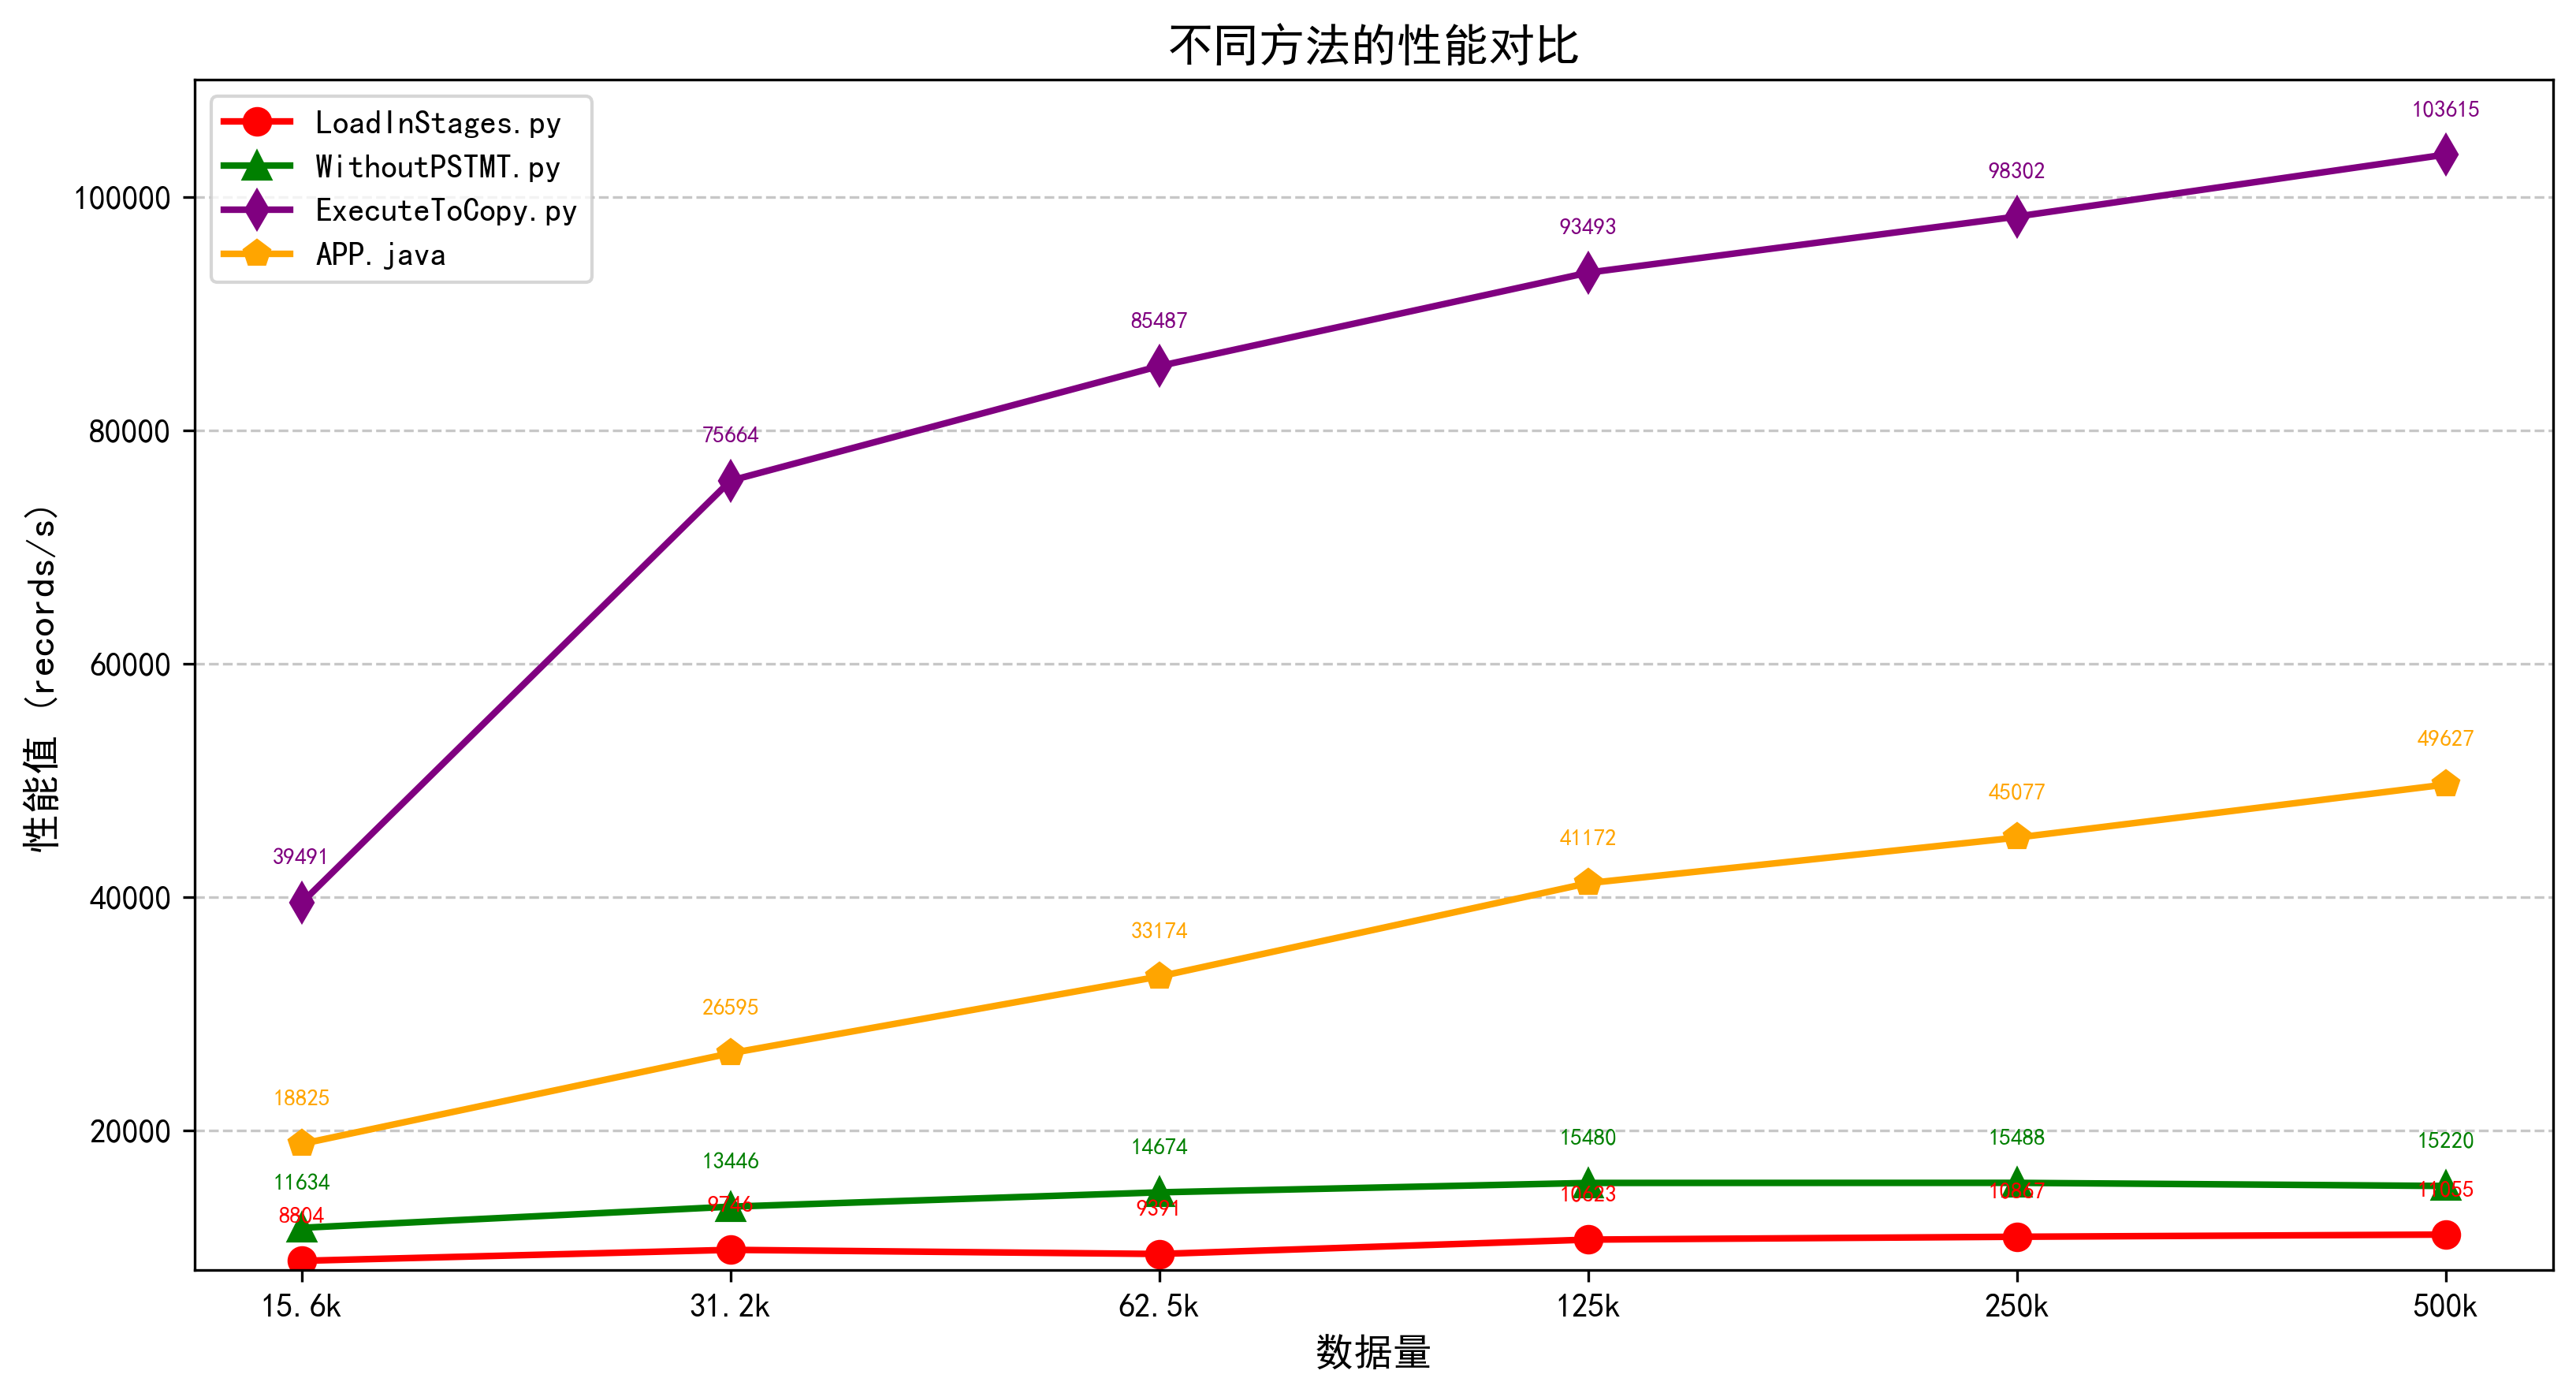
\includegraphics[width=1\textwidth]{volumes.png}
  \caption{不同数据量对于导入性能的影响}
  \label{fig:volume_performance}
\end{figure}

总体趋势而言，所有方法在15625的数据量下的性能均处于最低值，而随着数据量的增加，不同方法的导入性能均有所提升。考虑连接数据库与创建哈希Map等固定开销在数据量较小的情况下会有较大占比，导致性能偏低。而随着数据量的提升，固定开销的权重被插入数据稀释，使得性能呈上升趋势。\par
\hspace{0em}除此之外，可以发现第三次优化后的App.java以及ExecuteToCopy.py的性能提升最为显著。原因在于App使用的优化JDBC批量处理，以及ExecuteToCopy使用的copy方法下的单条记录插入时间极低，显著小于其他方法的单条记录插入时间。而随着数据量的提升，权重更多分配与导入速度，于是增幅最大，上升最为显著。具体细节已在4.3.2优化部分进行说明。\par

\subsubsection{trigger对于数据导入的影响}
PostgresSQL在Insert时会触发默认的约束检查，属于内部触发器。现在用Disable trigger all的sql语句进行触发器禁用。
其实实现方式与Python第一次优化类似，但是当时没有取消主键依赖，现在可以进一步禁用主键约束检查的触发器。对LoadInStages.py进行修改，添加禁用触发器的SQL语句，测试性能差异。\par
\hspace{0em}   able：9793 records/s\par
\hspace{0em}disable: 12290 records/s\par
性能提升了25.5\%，说明此方法能有效提升性能。但是这样插入数据易导致数据传入错误，极其不安全。本项目的Python优化是先导入再检查约束，均没有爆出异常，说明数据安全传入。


\end{document}